\documentclass[11pt]{article}

% ---------- Packages ----------
\usepackage[a4paper,margin=2.3cm]{geometry}
\usepackage[utf8]{inputenc}
\usepackage[T1]{fontenc}
\usepackage{lmodern}
\usepackage{textcomp}
\usepackage{graphicx}
\usepackage{booktabs}
\usepackage{array}
\usepackage{amsmath}
\usepackage{caption}
\usepackage{subcaption}
\usepackage[dvipsnames]{xcolor}
\usepackage[hidelinks, colorlinks=true, linkcolor=black, citecolor=black, urlcolor=NavyBlue]{hyperref}
\usepackage{enumitem}
\usepackage{fancyhdr}
\usepackage{titlesec}
\usepackage{float}
\usepackage{siunitx}

% ---------- Look and feel ----------
\titleformat{\section}{\normalfont\Large\bfseries}{\thesection.}{0.5em}{}
\titleformat{\subsection}{\normalfont\large\bfseries}{\thesubsection}{0.5em}{}
\setlist[itemize]{topsep=2pt, itemsep=1pt, parsep=0pt}
\setlist[enumerate]{topsep=2pt, itemsep=1pt, parsep=0pt}

\pagestyle{fancy}
\fancyhf{}
\renewcommand{\headrulewidth}{0.4pt}
\fancyhead[L]{\small Transfer Fee Valuation Engine}
\fancyhead[R]{\small Introduction to Machine Learning --- Group Project}
\fancyfoot[C]{\small\thepage}

\newcommand{\figwidth}{0.95\linewidth}

\title{\vspace{-1.5cm}\textbf{A Transfer Fee Valuation Engine}\\[2mm]
\large Pricing football transfers beyond the Transfermarkt market value}
\author{%
% TODO: replace with the five group members' names
Camille Auvity \quad Martin Loeul \quad Nils Quentin \quad Alexis Delisle \quad Iheb Ben Yakhlef \\[1mm]
\small MSc in Financial Engineering --- Introduction to Machine Learning, 2026--2027
}
\date{\today}

\begin{document}
\maketitle
\thispagestyle{fancy}
\vspace{-0.8cm}

\begin{abstract}
\noindent
Football clubs, agents and investors routinely use Transfermarkt's crowd\nobreakdash-sourced
market value as a quick, free estimate of what a transfer should cost. We build a
\textbf{pricing engine} that corrects this naive estimate using machine learning,
trained on 16{,}439 transfers (2005--2026) from the Transfermarkt panel. Modelling
the log fee\slash value ratio with a tuned XGBoost model, evaluated strictly
out\nobreakdash-of\nobreakdash-sample on the most recent 20\% of transfers, we
raise $R^2$ on the log fee from 0.738 (Transfermarkt alone) to 0.825, cut the
median pricing error from 47.1\% to 37.5\%, and beat the naive benchmark on
60.2\% of test transfers --- consistently across every period of the two-year
test window. We also show where the product should \emph{not} be trusted:
goalkeepers and transfers to Spanish clubs remain structurally mispriced, and
two natural refinements (error calibration, a neural network with club
embeddings) failed to close that gap.
\end{abstract}

% ======================================================================
\section{The Product}
% ======================================================================

\paragraph{The problem.} Every time a club considers buying or selling a player,
someone has to answer the question \emph{``what is this transfer actually
worth?''}. The industry's default answer is Transfermarkt's publicly listed
market value: a crowd-sourced estimate, free, instantly available, and
widely quoted in the media and in early-stage negotiations. It is also a
\emph{naive} estimate --- a single number that ignores recent form, contract
situation, the buying and selling clubs' financial context, and the
negotiating dynamics of the specific transfer window.

\paragraph{The product.} We build a \textbf{transfer fee valuation engine}: given
a player and a transfer context (age, position, recent performance, contract
length, selling and buying clubs), it predicts the fee the transfer should
command, expressed both as a corrected euro amount and as a premium or
discount relative to the Transfermarkt value.

\paragraph{How it works, concretely.} A recruitment analyst preparing a bid
enters the same handful of facts already on a player's profile sheet: age,
position, recent playing time and output, months left on contract, and the
selling and prospective buying clubs. The engine returns a corrected
transfer-fee estimate alongside the raw Transfermarkt figure, so the user
sees both numbers and the size of the gap between them --- turning a single,
static valuation into a range the club can defend at the negotiating table,
and a flag (``likely premium'' or ``likely discount'') the user can act on
before even looking at the exact amount.

\paragraph{The value, in numbers.} On the median transfer in our data
(\texteuro 1.5M), cutting the typical pricing error from 47\% to 37\%
(Section~5) is worth avoiding roughly \texteuro 140{,}000 of mispricing per
deal; for a club executing a dozen transfers a transfer window, that is a
material, recurring budgeting improvement, at the cost of nothing more than
the handful of inputs already collected for any serious recruitment file.

\paragraph{Who uses it, and for which decision.} The primary users are a club's
\textbf{recruitment and finance departments} on the buying side, and
\textbf{sporting directors} on the selling side:
\begin{itemize}
    \item \emph{Buying club}: is the asking price for a target reasonable, or is
    the player over-priced relative to what comparable transfers have actually
    cost? This feeds directly into transfer-window budget planning.
    \item \emph{Selling club}: what is a defensible floor for negotiations,
    beyond ``what Transfermarkt says''?
    \item \emph{Agents and intermediaries}: a data-driven anchor for
    negotiations, complementing (not replacing) their market knowledge.
\end{itemize}

\paragraph{What it replaces.} The product does not replace human judgement or
due diligence; it replaces the implicit \textbf{naive rule} ``final fee =
Transfermarkt market value'', which is exactly the benchmark we beat
throughout this report (Section~4). This benchmark is not a straw man: it is
the number that is actually quoted by journalists, used as a first anchor in
negotiations, and --- as we show in Section~5 --- it is wrong by a median of
47\% of the transfer amount.

% ======================================================================
\section{The Data}
% ======================================================================

\subsection{Source and unit of observation}
We use the \emph{Transfermarkt} dataset published on Kaggle
(\href{https://www.kaggle.com/datasets/davidcariboo/player-scores}{\texttt{davidcariboo/player-scores}}),
an openly documented panel of football transfers, player valuations, and
club information, which we enrich into a single \textbf{transfer-level panel}.
The unit of observation is \textbf{one transfer} (a player moving from a
selling club to a buying club on a given date), augmented with:
\begin{itemize}
    \item the player's characteristics at the time of the transfer (age,
    position, foot, nationality, international caps);
    \item the player's performance over the preceding 12 months (minutes
    played, goals, assists, cards, appearances);
    \item the player's transfer history (number of prior transfers, previous
    fee, previous market value);
    \item the selling and buying clubs' characteristics (squad size, average
    age, share of foreign players, number of national-team players, league,
    confederation, net transfer spending).
\end{itemize}
This gives \textbf{58 raw fields} before any feature engineering (well above
the 15-feature requirement), spanning transfers from \textbf{1 January 2005 to
1 January 2027}.

\subsection{Descriptive statistics}
After keeping only transfers with a disclosed, strictly positive fee and a
known Transfermarkt value, we obtain \textbf{16{,}439 transfers}. Table~\ref{tab:descriptive}
summarises the key variables; both the fee and the market value are heavily
right-skewed (a small number of transfers exceed \texteuro{}100M, while the median
is \texteuro{}1.5M), which motivates the modelling choice in Section~3.

\begin{table}[H]
\centering
\caption{Descriptive statistics of the transfer panel (N = 16{,}439).}
\label{tab:descriptive}
\begin{tabular}{lrrrrr}
\toprule
Variable & Mean & Std.\ dev. & Median & p25 & p75 \\
\midrule
Transfer fee (\texteuro{}) & 5.06M & 10.12M & 1.50M & 0.50M & 5.00M \\
Market value (\texteuro{}) & 4.59M & 8.74M & 1.50M & 0.60M & 4.50M \\
Age at transfer (years) & 24.0 & 3.4 & 23.6 & 21.5 & 26.1 \\
\bottomrule
\end{tabular}
\end{table}
\vspace{-2mm}
\noindent By position: 5{,}693 attackers, 4{,}959 defenders, 4{,}688 midfielders and
1{,}099 goalkeepers. By destination league: 1{,}646 Premier League, 1{,}575
Serie~A, 1{,}189 Bundesliga, 988 Ligue~1, 880 La Liga, and 10{,}161 to all
other leagues combined.

\subsection{Preparation steps}
\begin{enumerate}
    \item \textbf{Merge} the transfer panel with club-level data for both the
    selling and the buying club (squad size, average age, foreign-player
    share, national-team players, net transfer record).
    \item \textbf{Chronological lag feature}: for each player, the market value
    recorded at the \emph{previous} transfer is attached as a feature ---
    computed with a time-ordered \texttt{groupby} shift, never using a future
    transfer.
    \item \textbf{League bucketing}: the five ``Big 5'' domestic leagues are
    kept individually; all others are grouped as \texttt{Other}, to avoid a
    very sparse, high-cardinality categorical variable.
    \item \textbf{Encoding}: position, foot, league and confederation are
    one-hot encoded.
    \item \textbf{Target construction}: we define
    $\texttt{log\_spread} = \ln\!\left(\dfrac{\text{fee}}{\text{market value}}\right)$,
    the log premium (or discount) paid relative to the Transfermarkt value ---
    see Section~3 for the rationale. The top and bottom 2\% of
    \texttt{log\_spread} are trimmed as data-entry outliers, leaving
    \textbf{15{,}760 transfers}.
    \item \textbf{Missingness flags}: rather than dropping rows with a missing
    contract length, prior fee or value-momentum feature, we add an explicit
    \texttt{is\_missing\_*} indicator and impute, so that ``no information
    available'' is itself a feature the model can use.
\end{enumerate}

\begin{figure}[H]
\centering
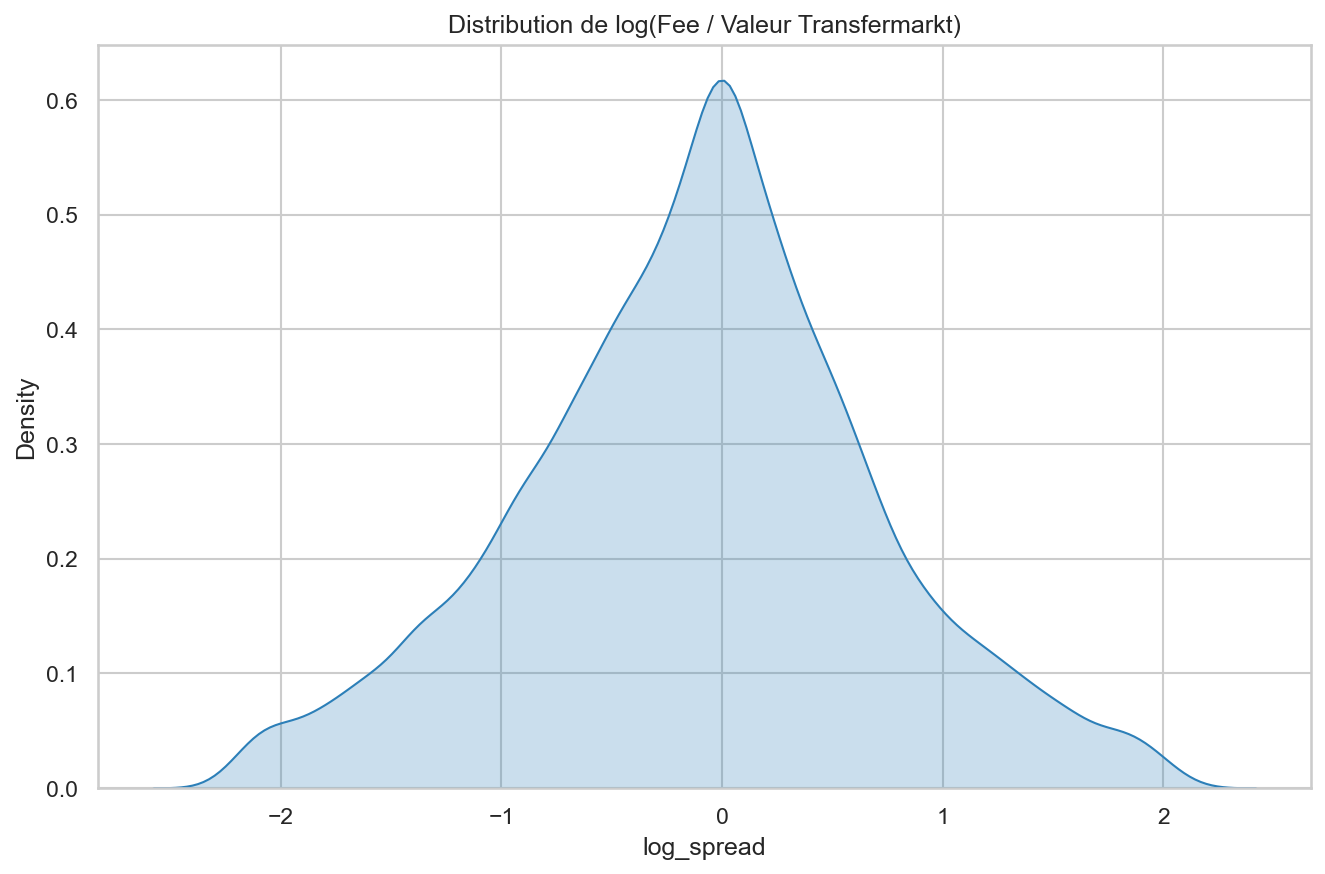
\includegraphics[width=0.55\linewidth]{figures/log_spread_distribution.png}
\caption{Distribution of the target variable, $\log(\text{fee}/\text{market value})$,
after trimming. Centred near zero (fee close to market value), with fatter
tails on the premium side.}
\label{fig:target_dist}
\end{figure}

\subsection{Related work}
Statistical modelling of football transfer fees is an established research
area. Poli et al. (2024) build a multiple linear regression on 8{,}389
worldwide permanent transfers (2014--2024), using contract length, age,
recent performance, position and the buying/selling clubs' economic
potential to explain $\log(\text{fee})$ directly, reaching $R^2 = 0.848$.
Their result is not directly comparable to ours: they predict the fee from
scratch, whereas our benchmark --- the Transfermarkt value --- already
captures much of that same signal, so our model is set the harder task of
explaining the \emph{residual} left once a strong naive estimate is already
on the table. Consistent with their findings that contract length and recent
form are first-order drivers, our own feature set includes both (years to
contract expiration, last-12-month performance); McHale and Holmes (2022) is
the closest machine-learning precedent, estimating transfer fees with
gradient boosting rather than linear regression. A further avenue we did not
pursue is the ``sporting level'' adjustment used by Poli et al. (2024), who weight a
player's minutes by the strength of the opposition faced; a dataset such as
the historical international results panel on Kaggle
(\href{https://www.kaggle.com/datasets/martj42/international-football-results-from-1872-to-2017}{\texttt{martj42/international-football-results}})
could support a similar feature in future work.

% ======================================================================
\section{The Methods}
% ======================================================================

\subsection{Target: a log fee-to-value ratio, not the raw fee}
We do not model the transfer fee directly. Fees range from \texteuro{}500 to
\texteuro{}222M, so a model minimising squared error on raw euros would be
entirely driven by a handful of blockbuster transfers. Instead we model
$\texttt{log\_spread} = \ln(\text{fee}) - \ln(\text{market value})$:
\begin{itemize}
    \item it is the log of a \emph{ratio}, so a \texteuro{}1M transfer priced 20\%
    above value and a \texteuro{}50M transfer priced 20\% above value contribute
    equally to the loss;
    \item it has a natural, interpretable benchmark: $\texttt{log\_spread}=0$
    means ``fee equals the Transfermarkt value'', which \emph{is} the naive
    rule we compete against;
    \item the final euro prediction is simply recovered as
    $\widehat{\text{fee}} = \text{market value} \times e^{\widehat{\texttt{log\_spread}}}$.
\end{itemize}

\subsection{Models}
We compare two families (Table~\ref{tab:models}): regularised linear models,
as an interpretable baseline, and tree-based ensembles, better suited to the
non-linear, interaction-heavy relationships we expect between e.g.\ age,
recent form and league. All models receive the same 43 features (after
encoding); the imputation and scaling needed by the linear models are fit on
the training fold only, inside a \texttt{scikit-learn} pipeline, to avoid any
leakage from the validation folds.

\begin{table}[H]
\centering
\caption{Models compared, and the key assumption each one makes about the data.}
\label{tab:models}
\small
\begin{tabular}{@{}p{3.3cm}p{5.4cm}p{6cm}@{}}
\toprule
Model & What it assumes & Why we include it \\
\midrule
Ridge / ElasticNet & Linear, additive effect of each feature; needs
scaling and imputation & Transparent, stable baseline; ElasticNet also
performs feature selection \\
Huber regression & Linear, but down-weights large residuals & Robust
baseline against fee outliers \\
Random Forest & Non-linear, no distributional assumption; needs imputed
inputs & Captures interactions without manual feature crossing \\
HistGradientBoosting, LightGBM, XGBoost, CatBoost & Non-linear,
sequentially corrects residuals; handles missing values natively &
State of the art on tabular data of this size; our main candidates \\
\bottomrule
\end{tabular}
\end{table}

\subsection{Why gradient boosting, and why XGBoost}
\textbf{Why not a linear model.} The relationship between a player's profile
and the premium paid is not additive: a short remaining contract depresses
the fee far more for a squad player than for a star the buying club cannot
afford to lose; a young age helps a promising attacker much more than a
promising full-back. Capturing this would require us to hand-build dozens of
interaction terms; a tree-based model discovers them on its own.

\textbf{How a gradient-boosted tree works.} XGBoost grows an ensemble of
shallow decision trees \emph{sequentially}: each new tree is fit not to the
target itself, but to the error still left by all the previous trees
combined, so the ensemble progressively corrects its own mistakes. Overfitting
--- a real risk on 12{,}608 training rows --- is controlled by shrinking each
tree's contribution (\texttt{learning\_rate}), limiting tree depth, and
penalising large leaf weights through an $\ell_2$ term
(\texttt{reg\_lambda}); the final prediction is simply the sum of every
tree's small correction.

\textbf{Why XGBoost specifically.} All four boosted-tree implementations we
tried land within a narrow band (test $R^2$(log fee) between 0.821 and
0.825, Table~\ref{tab:results}), so no single one is categorically the right
choice; the decision came down to three practical points. First, like
LightGBM, HistGradientBoosting and CatBoost --- but unlike Random Forest ---
XGBoost handles missing values natively, which matters here because several
engineered features (years to contract expiration, the previous transfer's
fee, value momentum) are missing for a meaningful share of transfers;
Random Forest needed an explicit median-imputation step and ended up the
weakest of the five non-linear models. Second, its \texttt{reg\_lambda}
regularisation combined with a pseudo-Huber loss proved a good match for our
outlier-heavy target, down-weighting the handful of blockbuster transfers
without discarding them as linear models' squared-error loss would.
Third, after the hyperparameter search described below, it came out
marginally but consistently ahead of the other three on every metric we
track (Section~5.1) --- a small edge, but the most reliable one we found.

\subsection{Respecting time: how we avoided look-ahead bias}
Because transfers are ordered in time and the economics of the transfer
market drift (inflation, COVID-19, new ownership rules), \textbf{every
evaluation in this project uses a chronological split, never a random one}:
\begin{itemize}
    \item the headline \textbf{train/test split is 80/20 in time}: the oldest
    12{,}608 transfers (up to 19 December 2024) train the models; the most
    recent 3{,}152 transfers are held out as the test set and are touched
    \emph{exactly once}, to report final numbers;
    \item all \textbf{cross-validation}, for the linear models' regularisation
    strength and for the gradient-boosting hyperparameter search, uses
    \texttt{TimeSeriesSplit} (5 folds), which always validates on data that
    comes after the training fold, never on data that comes before it;
    \item the \textbf{hyperparameter search} (\texttt{RandomizedSearchCV}, 25
    draws per model, on XGBoost, LightGBM, HistGradientBoosting and Random
    Forest) is run \emph{only} on the training period; the resulting
    hyperparameters are then evaluated once on the untouched test period to
    confirm the gain survives out of sample (it does for three of the four
    models; LightGBM's original hyperparameters were kept, as tuning did not
    improve its test performance).
\end{itemize}

% ======================================================================
\section{The Evaluation}
% ======================================================================

\subsection{Metrics}
We report three complementary views of performance, all computed on the
untouched test set:
\begin{enumerate}
    \item \textbf{On the modelling scale}: MAE, RMSE and $R^2$ on
    \texttt{log\_spread} directly.
    \item \textbf{In business terms}: once converted back to euros, $R^2$ on
    $\log(\text{fee})$, MAE and RMSE in \texteuro{}M, the \textbf{median absolute
    percentage error} on the final fee, and the share of predictions within
    $\pm 20\%$ / $\pm 30\%$ of the true fee.
    \item \textbf{As a direction call}: a club often first wants to know
    \emph{whether} it is likely to pay a premium over Transfermarkt value
    before caring about the exact amount. We therefore also report accuracy,
    ROC-AUC, precision and recall of the model as a binary classifier of
    ``premium vs.\ discount''.
\end{enumerate}

\subsection{Benchmark}
The benchmark, throughout, is the \textbf{naive rule the product replaces}:
$\widehat{\texttt{log\_spread}} = 0$, i.e.\ ``the transfer fee will equal the
Transfermarkt market value''. This is not an arbitrary straw man --- it is
literally what a user would believe without our product.

\begin{figure}[H]
\centering
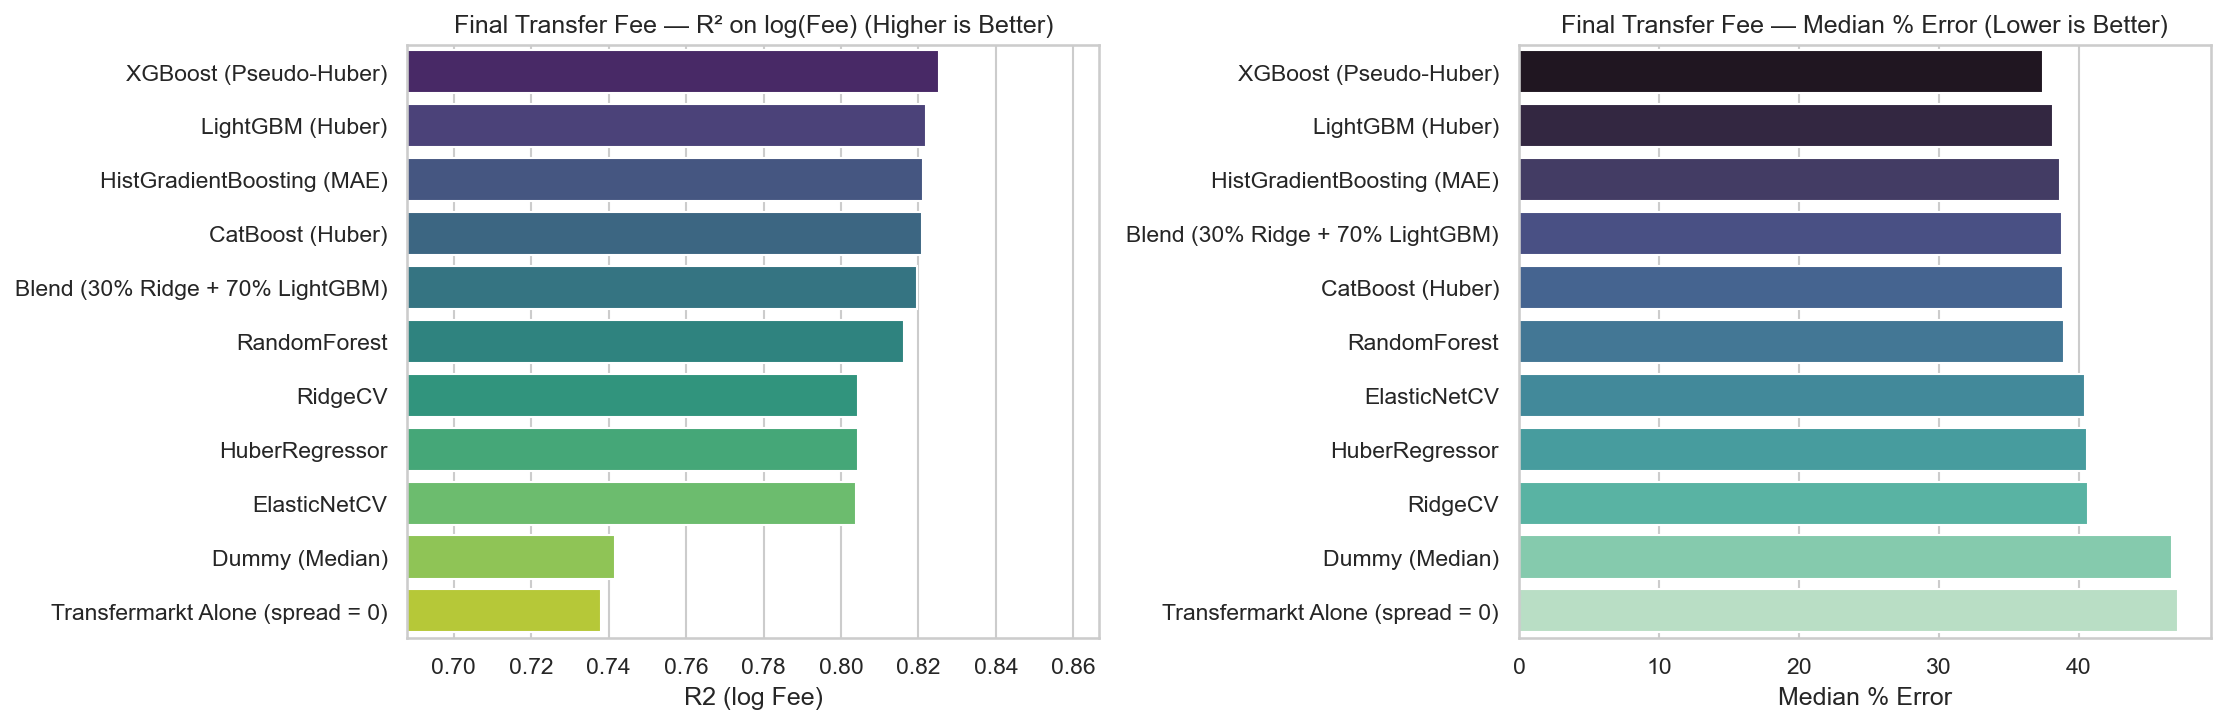
\includegraphics[width=0.78\linewidth]{figures/final_fee_comparison.png}
\caption{Out-of-sample performance of every model against the Transfermarkt
benchmark, on $R^2(\log \text{fee})$ (left, higher is better) and median
percentage error on the final fee (right, lower is better).}
\label{fig:final_comparison}
\end{figure}

\begin{figure}[H]
\centering
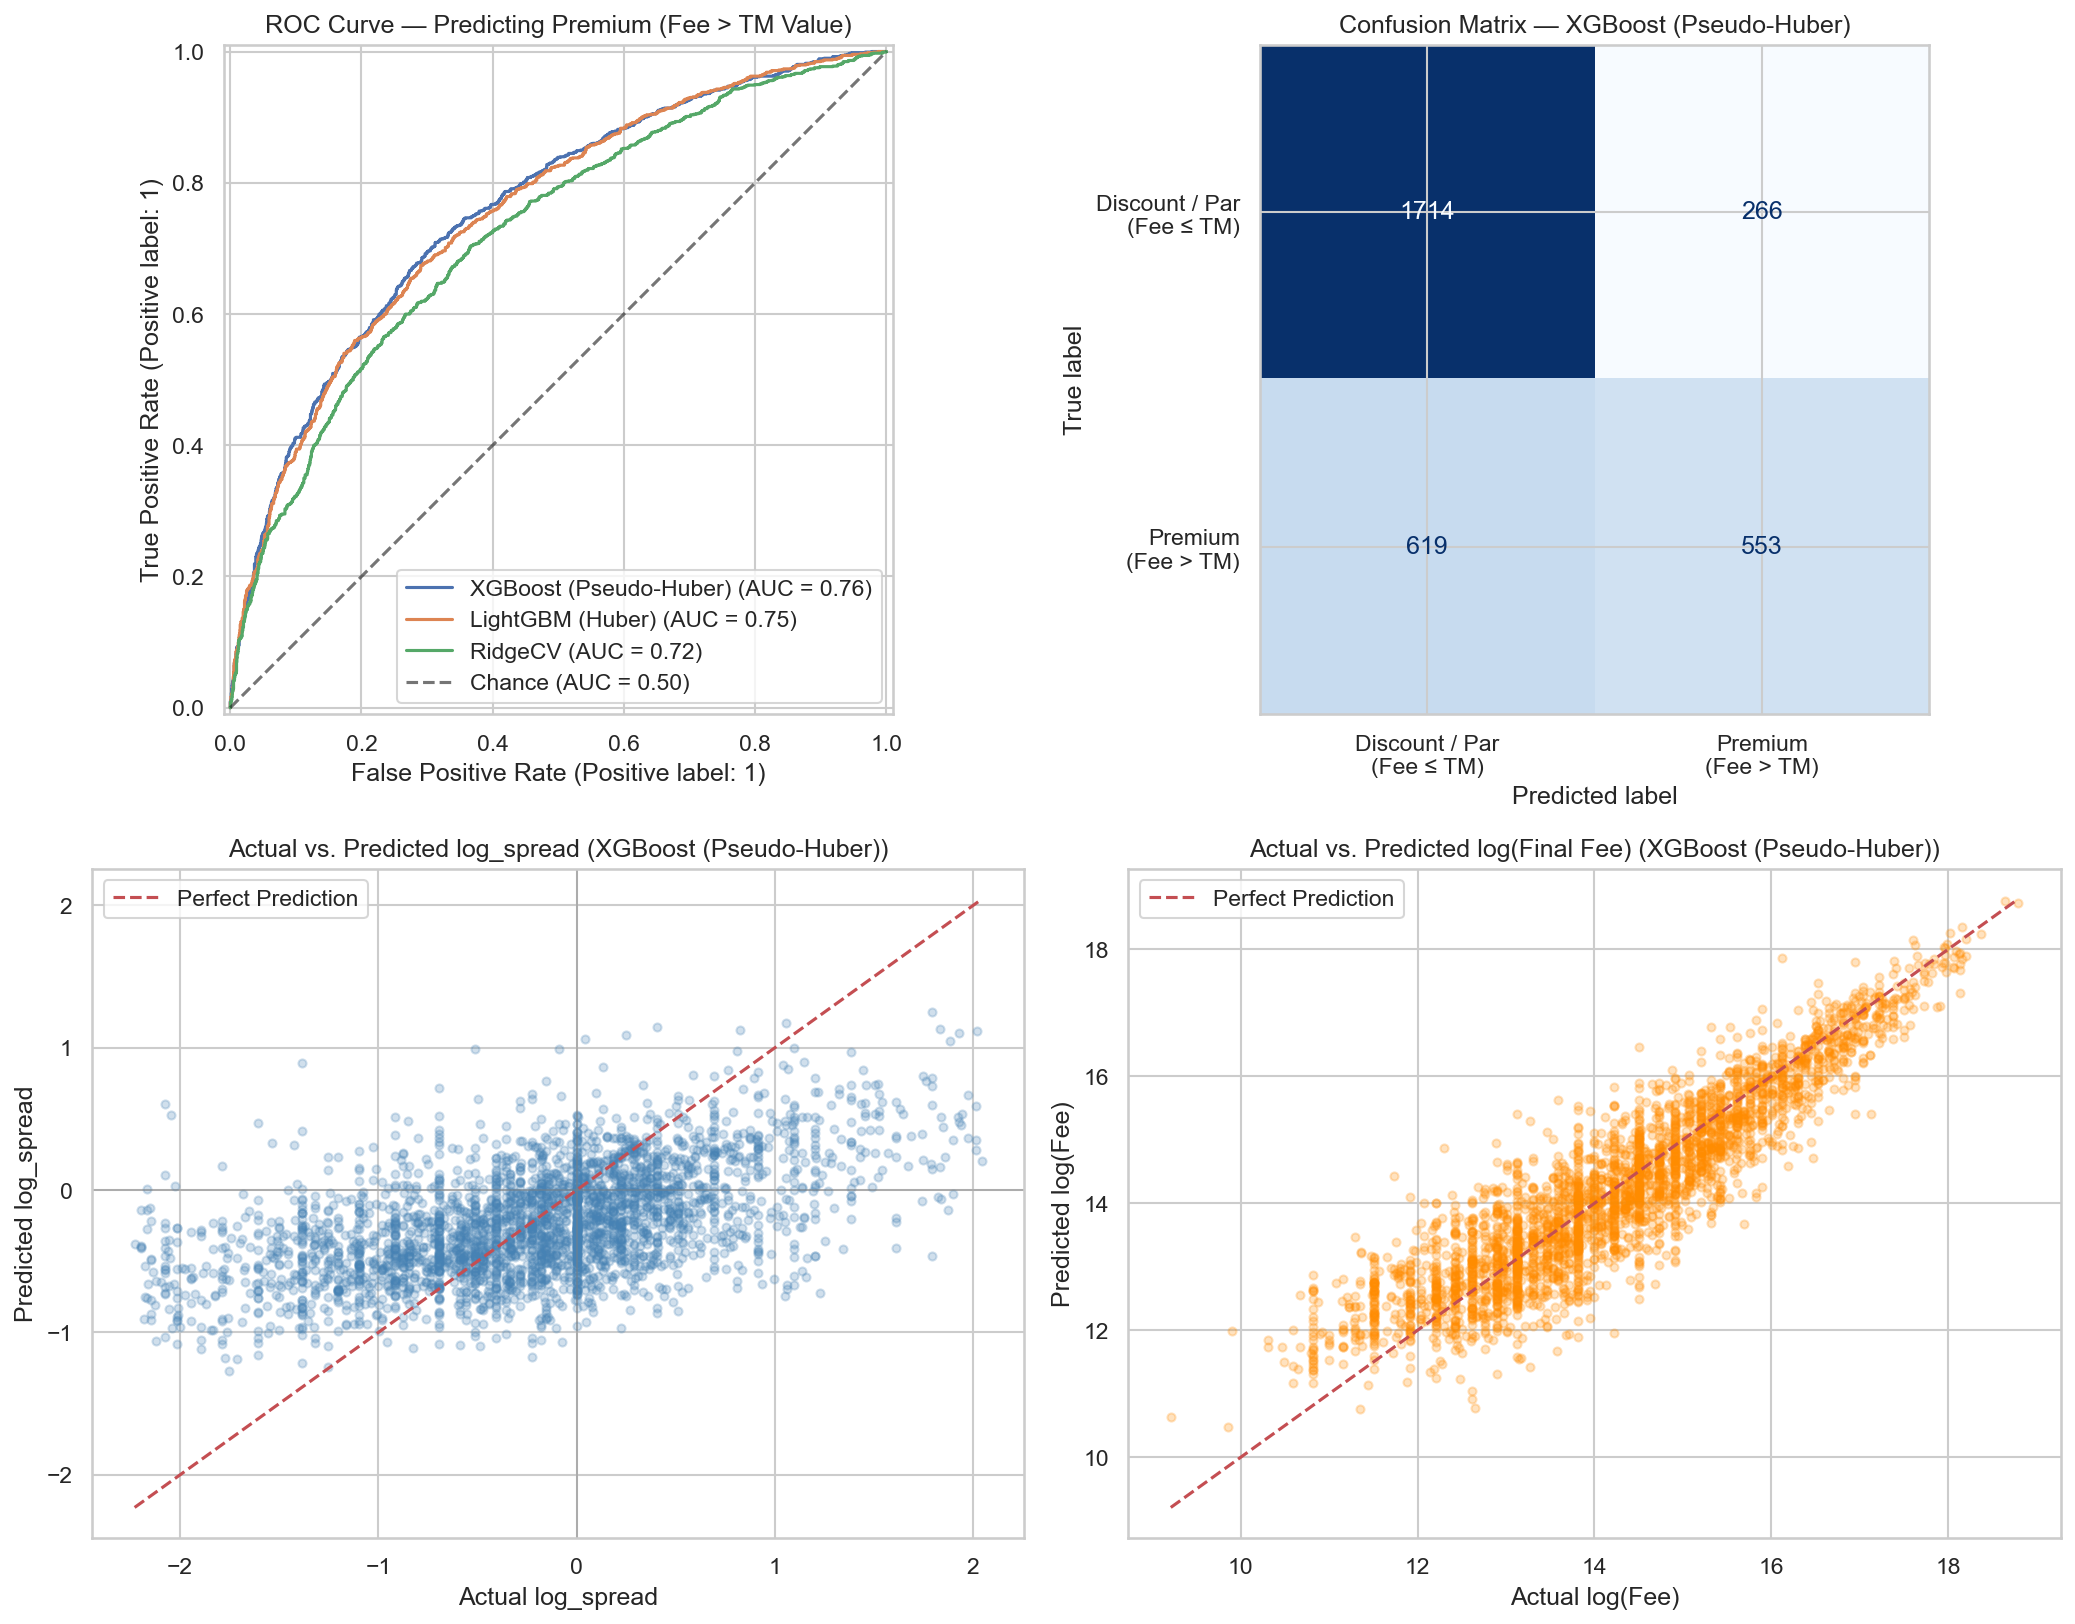
\includegraphics[width=0.66\linewidth]{figures/diagnostics_panel.png}
\caption{Diagnostics for the best model (tuned XGBoost): ROC curve for the
premium/discount classification (top left), confusion matrix (top right),
and actual vs.\ predicted values on the log-spread and log-fee scales
(bottom row). Points on the red dashed line are perfectly predicted.}
\label{fig:diagnostics}
\end{figure}

% ======================================================================
\section{Results and their Limits}
% ======================================================================

\subsection{Headline result}
Table~\ref{tab:results} reports the out-of-sample results for the main
models. The tuned \textbf{XGBoost} model is the best performer on every
metric we track, and is the model deployed in the product.

\begin{table}[H]
\centering
\caption{Out-of-sample performance (test set, N = 3{,}152 transfers).}
\label{tab:results}
\small
\begin{tabular}{lccccc}
\toprule
Model & $R^2$(log fee) & MAE (\texteuro{}M) & RMSE (\texteuro{}M) & Med.\ \% error & $\pm$30\% \\
\midrule
\textbf{XGBoost (tuned)} & \textbf{0.825} & \textbf{1.65} & \textbf{3.65} & \textbf{37.5\%} & \textbf{39.9\%} \\
LightGBM & 0.822 & 1.67 & 3.68 & 38.2\% & 39.0\% \\
HistGradientBoosting & 0.821 & 1.65 & 3.60 & 38.5\% & 39.4\% \\
Random Forest & 0.816 & 1.70 & 3.79 & 39.0\% & 39.4\% \\
RidgeCV (linear) & 0.805 & 1.82 & 4.26 & 40.7\% & 37.3\% \\
\midrule
\emph{Transfermarkt alone (benchmark)} & 0.738 & 1.89 & 4.09 & 47.1\% & 36.0\% \\
\bottomrule
\end{tabular}
\end{table}

\noindent The tuned XGBoost model improves $R^2$ on the log fee from 0.738 to
0.825, cuts the median pricing error from 47.1\% to 37.5\%, and
\textbf{beats the Transfermarkt value on 60.2\% of the test transfers}.
Hyperparameter tuning itself contributed only a modest share of this gain
(test MAE on \texttt{log\_spread} improved from 0.513 to 0.509): most of the
value comes from using a non-linear model at all, not from tuning it further.

\subsection{Where the product helps the most}
Figure~\ref{fig:tier} breaks the comparison down by Transfermarkt valuation
tier. The naive benchmark is worst precisely where the stakes are highest for
a club with a limited budget: transfers below \texteuro{}1M are mispriced by a
median of 60\% if one trusts Transfermarkt alone, against 47\% with our
model. For the largest transfers (above \texteuro{}15M), the market is already
fairly efficient (both the benchmark and the model are accurate), but our
model still raises the share of transfers priced within $\pm 30\%$ of the
truth from 62\% to 69\%.

\begin{figure}[H]
\centering
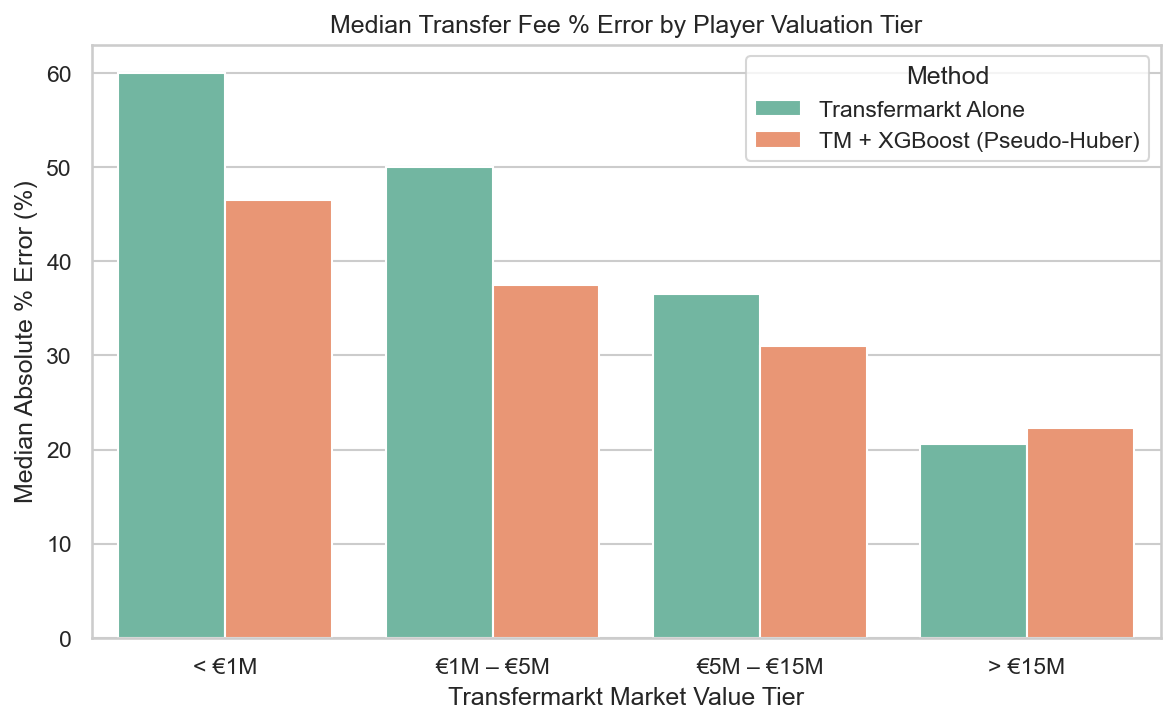
\includegraphics[width=0.52\linewidth]{figures/fee_error_by_valuation_tier.png}
\caption{Median pricing error, Transfermarkt alone vs.\ our model, by
valuation tier.}
\label{fig:tier}
\end{figure}

\subsection{Stability over time}
A product is only useful if its edge is not a lucky artefact of the
particular test window chosen. We split the roughly two-year test period
into ten equal-sized, consecutive windows and recompute the comparison in
each. The model beats the Transfermarkt benchmark in \textbf{every single
window}, with no sign of the advantage shrinking over time
(Figure~\ref{fig:over_time}).

\begin{figure}[H]
\centering
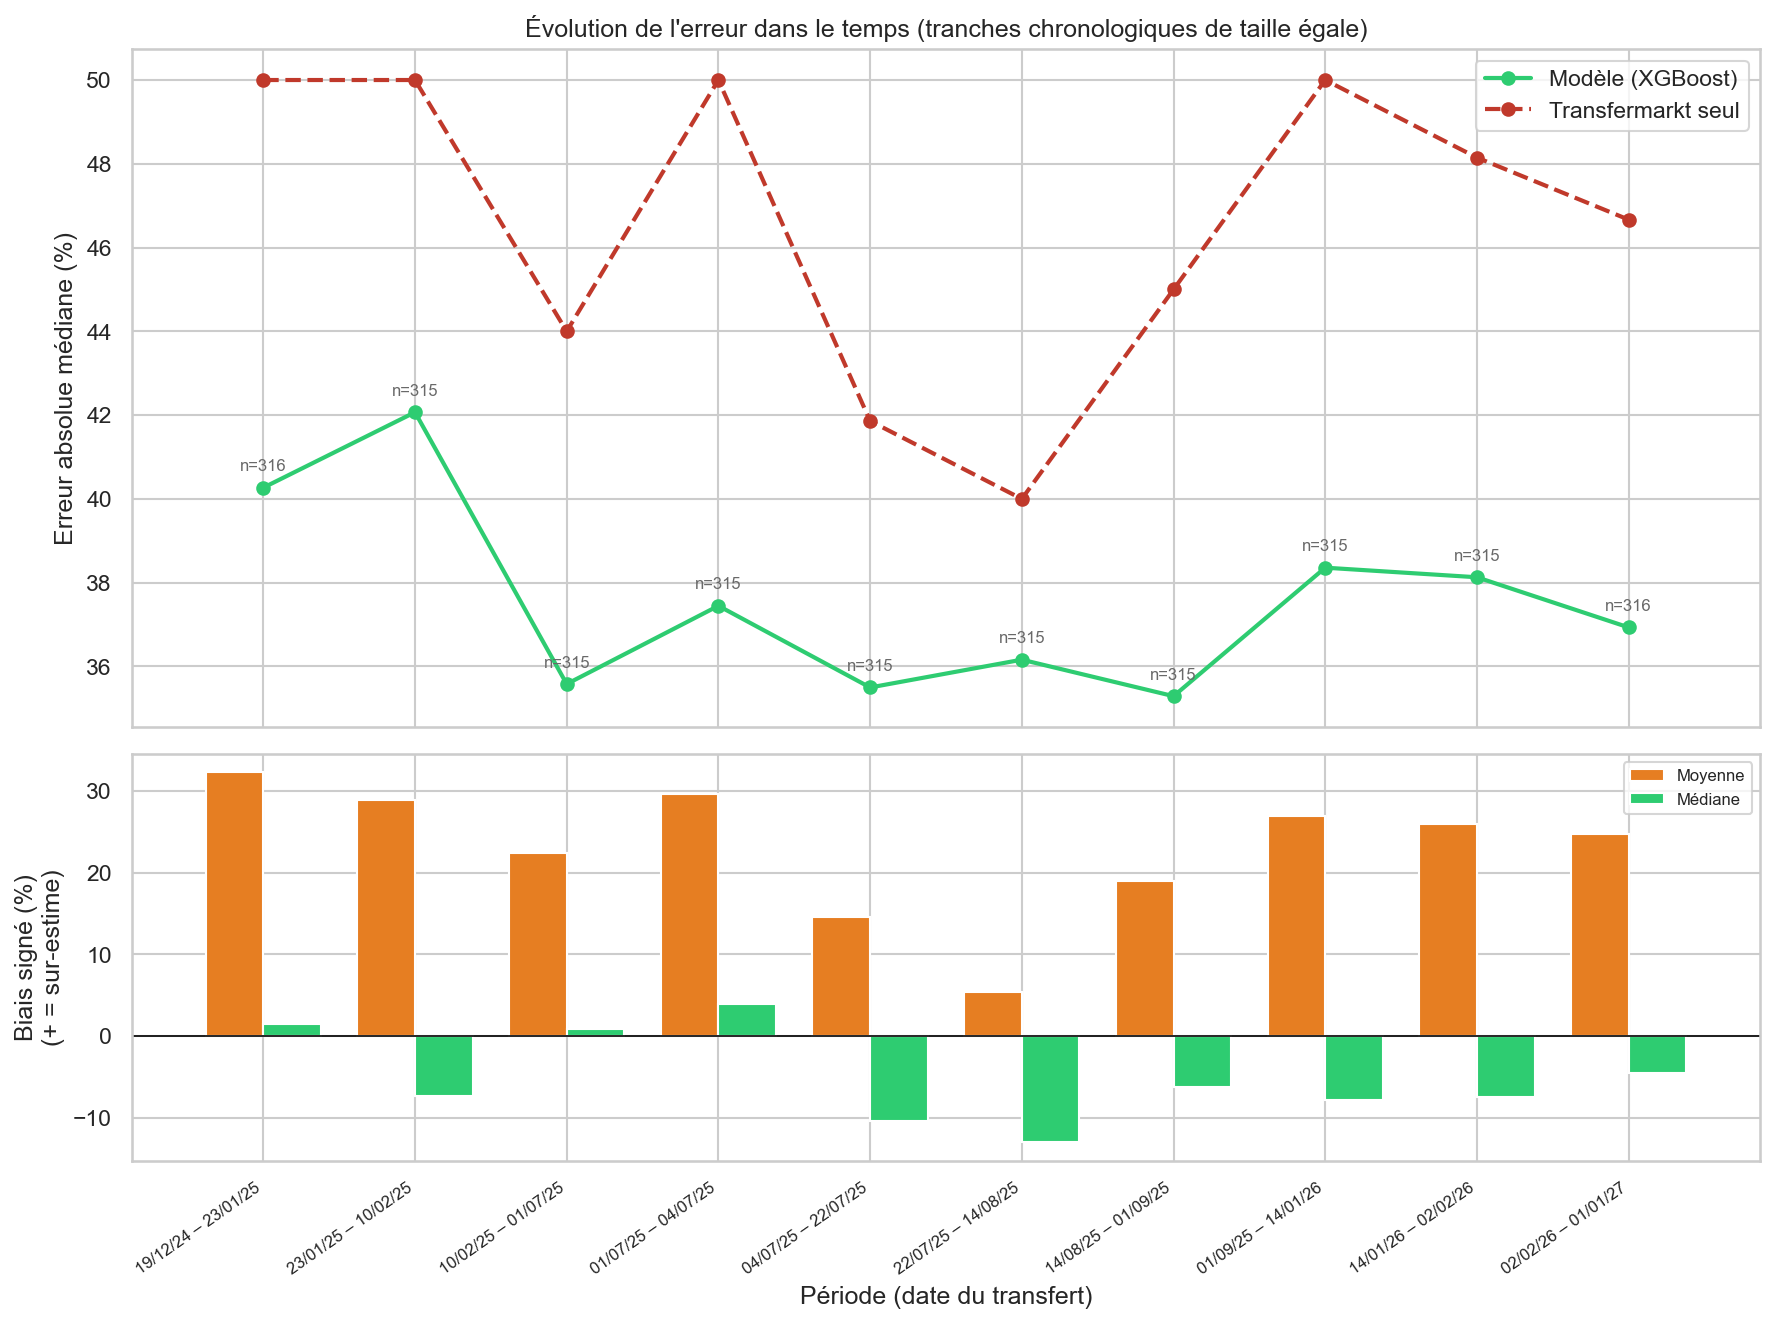
\includegraphics[width=0.64\linewidth]{figures/error_over_time.png}
\caption{Median pricing error over ten consecutive test-set windows: the
model (green) consistently beats Transfermarkt alone (red, dashed). Bottom
panel: average signed bias of the model is small and not systematically
drifting.}
\label{fig:over_time}
\end{figure}

\subsection{What drives the predictions, and what cannot be claimed}
Feature-importance analysis (not shown in detail here for space) confirms
that the Transfermarkt value itself, the player's age and recent playing
time, and the buying club's league are the dominant drivers --- the model
mostly \emph{refines} the existing valuation rather than replacing it with
an unrelated signal, which is reassuring for an industry user who already
trusts Transfermarkt as a starting point.

Looking at the \emph{median} (rather than the mean, which a handful of
very cheap, highly mis-priced transfers would distort) signed error by
segment, the model is close to unbiased almost everywhere, with two clear
exceptions:
\begin{itemize}
    \item \textbf{Goalkeepers} are over-priced by the model by a median of
    13.5\%, against $-5$ to $-7\%$ for outfield players --- the goalkeeper
    transfer market is thinner (1{,}099 of 16{,}439 transfers) and appears to
    follow different dynamics;
    \item transfers to \textbf{La Liga} clubs are over-priced by a median of
    10.0\%, while every other league is at or below 2\% --- consistent with
    Spanish clubs' well-documented financial constraints (La Liga's own
    spending controls), which push actual fees below what a generic model
    would expect.
\end{itemize}

\textbf{What the product cannot claim.} It cannot price a specific agent's
negotiating leverage, a release clause, or a club's idiosyncratic urgency to
sell or buy --- these are deal-specific facts absent from the data, and they
are plausibly a large part of the roughly 35--40\% of transfers that remain
outside our $\pm 30\%$ band. We tested two natural ways to close this
remaining gap and report them for completeness, without recommending either
for production: (i) a post-hoc isotonic calibration of the bias, which helps
the majority of segments but makes the goalkeeper and La Liga bias \emph{worse},
because it learns a single, global correction; and (ii) a small neural
network with learned club embeddings, intended to capture club-specific
pricing behaviour implicitly --- it under-performs XGBoost ($R^2=0.812$) and
does not close the La Liga gap, most likely because the $\sim$1{,}900
distinct clubs in the training data leave too few transfers per club for a
meaningful embedding. Both experiments, and the reasoning behind rejecting
them, are available in the code repository.

% ----------------------------------------------------------------------
\section*{Conclusion}
% ----------------------------------------------------------------------
A tuned XGBoost model, evaluated with a strict chronological split to avoid
any look-ahead bias, turns the industry's naive Transfermarkt valuation into
a materially better, consistently reliable pricing signal: $R^2$ rises from
0.738 to 0.825, the median pricing error falls from 47\% to 37\%, and the
gain holds across every segment of time we tested. The clearest next step is
not more model complexity --- tuning, calibration and even a neural network
all failed to move the needle much further --- but \textbf{richer data}:
club-level financial indicators (debt, Financial Fair Play status) to
explain the La Liga gap, and contractual details (release clauses, contract
length) to narrow the remaining unexplained variance.

\section*{References}
\begin{itemize}[leftmargin=1.4em]
    \item Poli, R., Besson, R., and Ravenel, L. (2024). Statistical Modeling
    of Football Players' Transfer Fees Worldwide. \textit{International
    Journal of Financial Studies}, 12(3), 93.
    \url{https://doi.org/10.3390/ijfs12030093}
    \item McHale, I., and Holmes, B. (2022). Estimating transfer fees of
    professional footballers using advanced performance metrics and machine
    learning. \textit{European Journal of Operational Research}, 306,
    389--399.
    \item davidcariboo (2024). Player Scores [Data set]. Kaggle.
    \url{https://www.kaggle.com/datasets/davidcariboo/player-scores}
    (primary dataset used in this project, see Section 2).
    \item martj42 (2019). International football results from 1872 to 2017
    [Data set]. Kaggle.
    \url{https://www.kaggle.com/datasets/martj42/international-football-results-from-1872-to-2017}
    (not used in the current pipeline; a candidate source for a future
    ``opposition strength'' feature, see Section 2.4).
    \item \textit{[To be completed: course reference(s) in data science
    followed by Camille Auvity and Martin Loeul --- institution and exact
    course title(s)]}.
\end{itemize}

\clearpage
\appendix
\section*{Appendix}

\subsection*{A. Contribution statement}
\textit{[To be completed and signed by the five group members: who worked on
data preparation, modelling, evaluation, the report, and the two
presentations.]}

\subsection*{B. Use of AI tools}
We used \textbf{Claude Code} (Anthropic) as a coding and analysis assistant
throughout the project, under human direction and review at every step. Its
main uses were:
\begin{itemize}[leftmargin=1.4em]
    \item \textbf{Converting} our exploratory Jupyter notebook into the
    modular \texttt{src/} pipeline used for this report, without changing
    the underlying modelling logic;
    \item \textbf{Extending the analysis}: implementing the hyperparameter
    search (\texttt{tune\_models.py}), the segment- and time-based error
    analysis (\texttt{error\_analysis.py}), and the two rejected refinements
    discussed in Section 5.4 (isotonic calibration, the club-embedding
    neural network);
    \item \textbf{Critiquing our own results}: at several points the
    assistant flagged that a conclusion drawn from the \emph{mean} signed
    error was an artefact of outliers and re-derived it with the median,
    materially changing what we report in Section 5.4;
    \item \textbf{Drafting this report} from the project's code, saved
    tables and figures.
\end{itemize}
Every reported number was checked by re-running the corresponding script
end-to-end and comparing the console output and the files written to
\texttt{outputs/tables/} and \texttt{outputs/figures/} against what is
written here; no figure in this report was generated by the assistant
without a matching artefact in the code repository.

\end{document}
